\section{Empirical Evaluation}
\label{sec:eval}

We implemented our technique in a prototype tool called \tool{} (BUSiness
TEsting Rules), and conducted two empirical studies using two open-source
applications and one proprietary enterprise application. In the first study, we
compared the effectiveness of \tool{} in covering business rules with a related
technique that systematically explores the search space without any guidance. In
the second study, we investigated the efficiency of both the techniques. After
describing the experimental setup, we present results of the two studies.

\begin{table}[t]
\caption{Subjects used in our empirical studies.}
\centering
{\scriptsize
\tabcolsep=3pt
\begin{tabular}{|l|l|r|r|r|r|}
\hline
\multicolumn{1}{|c|}{Subject} & \multicolumn{1}{|c|}{URL} & \multicolumn{1}{|c|}{Entities} & \multicolumn{1}{|c|}{Operations} & \multicolumn{1}{|c|}{Rules} & \multicolumn{1}{|c|}{Rule parts} \\
\hline \hline
Cebu-pacific & www.cebupacificair.com 		& 8  & 10 & 15	 & 31 \\
jBilling 		 & www.jbilling.com 					& 10 & 10 & 14 	 & 26 \\
App 				 & \multicolumn{1}{|c|}{---}	& 12 & 13 & 13   & 20 \\
\hline \hline
\textbf{Total} & 													& 	 & 33 & 42   & 77 \\
\hline
\end{tabular}
}
\label{tab:subjects}
\end{table}


\subsection{Experimental Setup}
\label{sec:impl}
\vspace*{-3pt}
\paragraph*{Implementation} Our implementation \tool{}  uses \choco{} constraint
solver~\cite{Choco} for checking the satisfiability of sequences. Since \choco{} does not provide
functionality for extracting unsatisfied core, we use a heuristic-based
implementation to extract the core. While checking whether a concrete sequence
is satisfiable, \tool{} starts with the last operation of the sequence and
performs backward analysis by handling each operation and their rule
parts. Therefore, when a composed formula is unsatisfiable, it can be caused
only by a constraint in the most recently analyzed rule part. Next,
it uses the variables involved in that constraint to extract the complete
unsatisfied core. Note that \tool{} may not extract the minimal unsatisfied
core; however, the extracted core is sufficient to suggest candidate
operations. We leave improvements in the implementation to future work, for
example, by exploring advanced algorithms for extracting unsatisfied
core~\cite{Liffiton:2008:ACM} and also leverage other constraint
solvers~\cite{DeMoura:2008}. Another optimization could include caching and
reusing constraints (\eg as discussed in the Green approach~\cite{VisserGD12})
to improve further the efficiency of the search.

To compare the efficiency of \tool{} with an unguided search
over the space of candidate sequences, we implemented another tool, called
\exhaust{}. \exhaust{} is primarily the same as \tool{} without optimizations
presented in Section~\ref{sec:optimization}. Being an unguided technique, \exhaust{} lets us evaluate the
effectiveness of leveraging unsatisfied core to guide the search for covering
sequences.

%that systematically explores sequences without guidance via
%unsatisfied core. Similar to \tool{}, \exhaust{} uses a queue $q$ to store
%candidate sequences. Given an operation ${\cal O}$ and a target rule part $r$,
%\exhaust{} first creates a sequence $seq$ with ${\cal O}\ [r]$ and adds $seq$ to
%$q$. For each $seq$, \exhaust{} associates a list of input entities, referred to
%as \subject{ilist}.  Initially, \subject{ilist} contains the input entities of
%${\cal O}$ only.  Next, \exhaust{} dequeues a sequence $qseq$ from $q$, removes
%an entity from \subject{ilist}, and identifies all operations \{${\cal O}_1,
%{\cal O}_2, \ldots, {\cal O}_n$\} that create or modify that entity. \exhaust{}
%creates new sequences by adding each ${\cal O}_i$ to $qseq$. Also, if an ${\cal
%  O}_i$ requires additional input entities, it adds those entities to the
%\subject{ilist} for the newly created sequence. Next, it adds the new sequences
%to $q$ and repeats the process. When \exhaust{} encounters a concrete sequence,
%\ie{} a sequence whose \subject{ilist} is empty, it uses \choco{} to check
%whether the sequence is satisfiable: if it is, \exhaust{} returns the sequence
%and terminates; otherwise, it continues analyzing other sequences in
%$q$. \exhaust{} repeats this process until it finds a satisfiable sequence or
%reaches the user-defined upper bound on the number of sequences to be explored. 

\paragraph*{Subjects and Rules} We used two open-source applications and a proprietary enterprise application,
listed in Table~\ref{tab:subjects}, as the experimental subjects. Due to
confidentiality reasons, we refer to the proprietary application as
\subject{App}. \subject{Cebu-pacific} is an airlines application,
\subject{jBilling} is an enterprise billing application, and \subject{App} is a
telecom application. Column~2 shows the URLs of the first two subjects.
Columns~3--6 show additional details, such as the number of entities,
operations, and rules. For each subject, we identified a module that is likely
to have large number of interesting rules with respect to the sequences and test
data required for coverage, and modeled those modules using our tool. In
particular, we used the \textit{ticket cancellation} and \textit{generate
  invoice} modules for \subject{Cebu-pacific} and \subject{jBilling},
respectively. In total, we modeled $33$ operations with $42$ rules and $77$ rule
parts.\footnote{\small The complete dataset including models and the
  generated test sequences is available at \url{http://tinyurl.com/k4b4j8x}
  (also available on request from the authors).} For each subject, we spent
approximately~10 hours to model the operations and rules. We also found that
our rule editor and property checking helped create correct rule set.

\paragraph*{Method} We applied \tool{} and \exhaust{} on the models created for each subject and
generated test sequences. For each rule part, we let each tool explore up to a
maximum of $100$ concrete sequences. Next, we inspected the generated sequences
to ensure that they cover the targeted rule parts. To evaluate the efficiency of
the tools, we measured the number of sequences explored and the lengths of
sequences produced by each tool.  All experiments were conducted on an Intel
Core 2 Duo CPU machine with 2.53 GHz and 8GB RAM. Next, we present the results
of the studies.

\subsection{Coverage of Business Rules}

\begin{figure}[t]
\centering
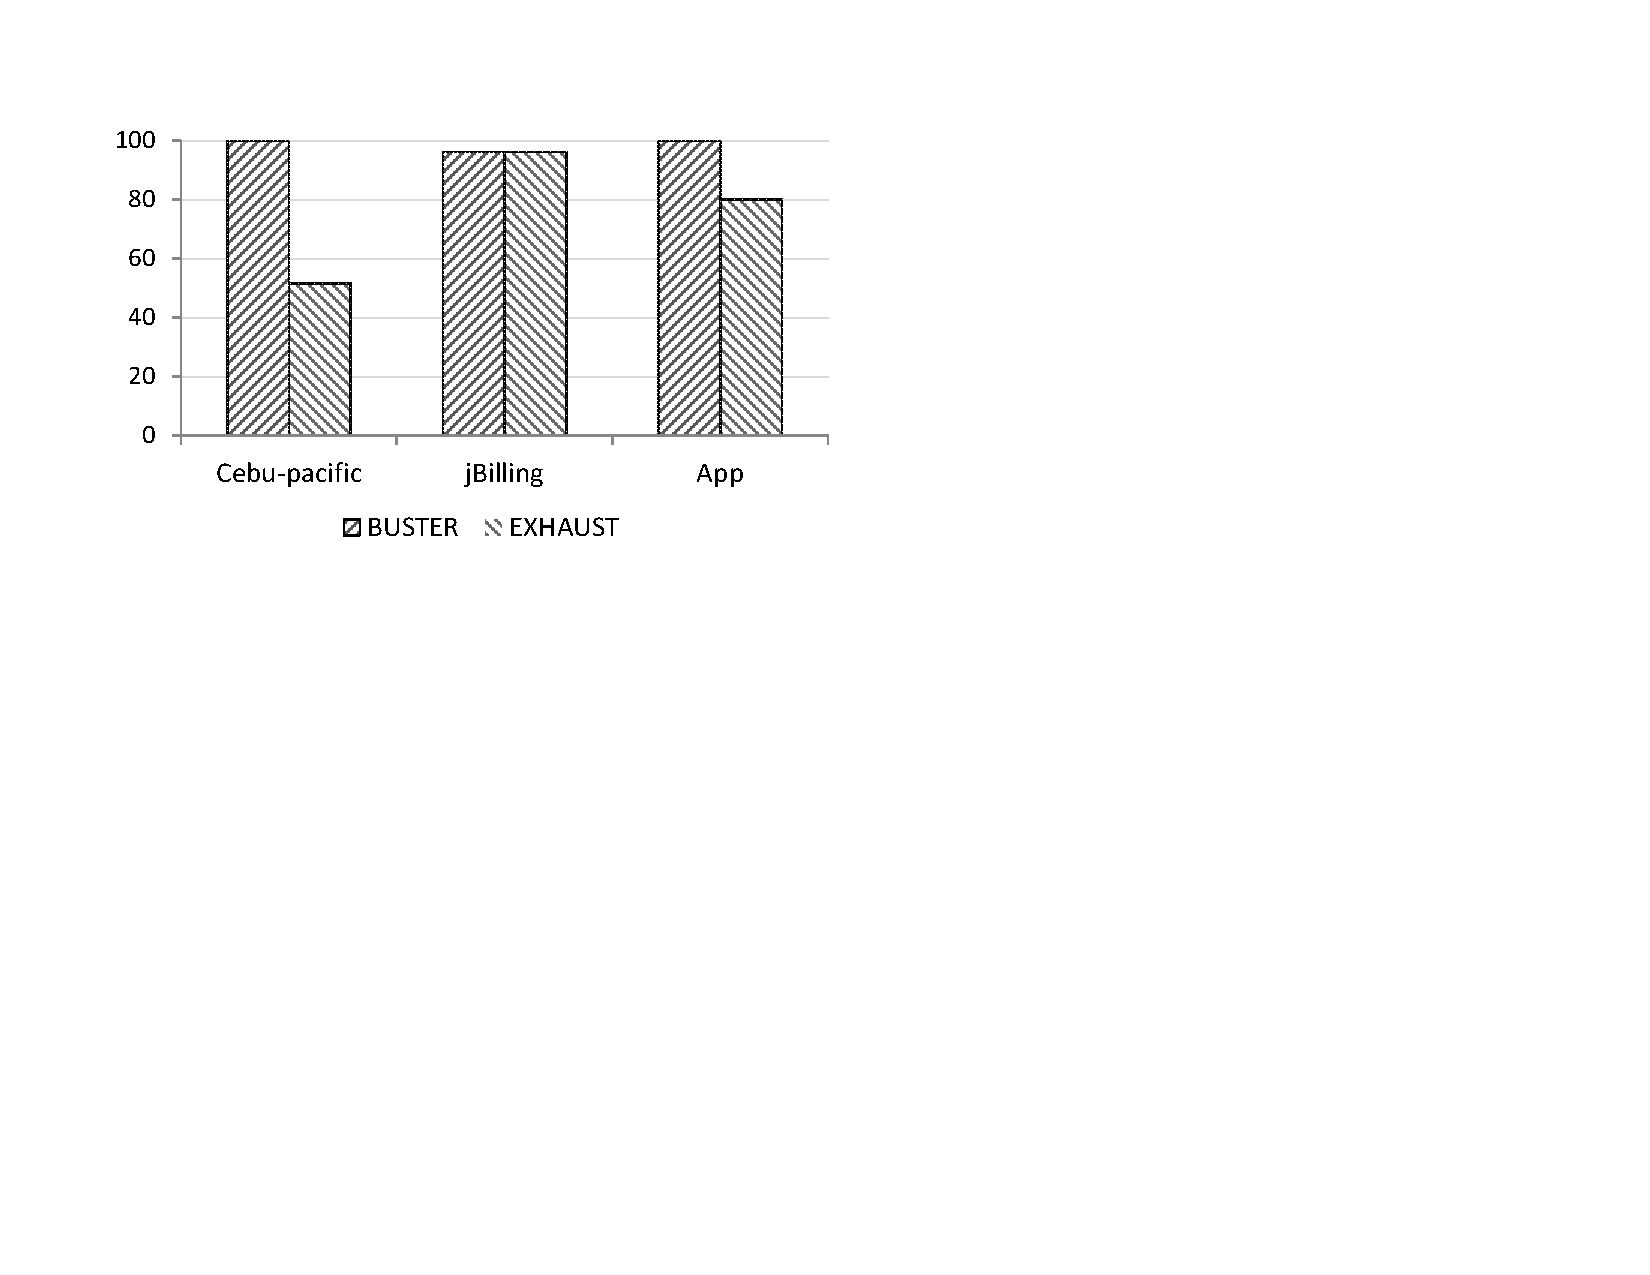
\includegraphics[width=0.65\columnwidth, clip, trim = 18mm 120mm 140mm
  18mm]{figs/Study-1.pdf}
\vspace*{-10pt}
\caption{Effectiveness of the two techniques in covering business rules.}
\label{fig:effectiveness}
\end{figure}

Figure~\ref{fig:effectiveness} presents the results for all three subjects: it
shows the percentages of rule parts covered by each tool. For example, for
\subject{Cebu-pacific}, \tool{} generated covering sequences for all $31$ rule
parts, whereas \exhaust{} was able to generate sequences only for $16$ rule
parts. Overall, the results show that \tool{} covered $99$\% of the rule parts,
whereas \exhaust{} could cover only $74$\% of the rule parts.

We further analyzed the cases where the tools could not cover the targeted rule
parts. We found that, in general, \exhaust{} performs poorly if there are many
operations that create or modify the required input entities. This is expected
because it results in a large search space of candidate operation sequences,
which \tool{} is able to navigate effectively in a goal-directed manner (guided
by the unsatisfied core), whereas \exhaust{} has to try the candidate sequences
in a blind manner. Thus, \exhaust{} performed well on \subject{jBilling}, in
which each entity is created or modified by only a few operations. But, for
\subject{Cebu-pacific}, where some entities are modified by many operations,
\exhaust{} was much less effective. In such cases, a directed search guided by
unsatisfied core, is necessary---and can be highly effective---for attaining
high rule coverage.

For \subject{jBilling}, both \tool{} and \exhaust{} could not cover one rule
part because of an issue with \choco{} solver: \choco{} terminated with an
out-of-memory error while solving the composed formula for that rule part.

%% While analyzing our results, we identified that the rule parts that were not
%% covered by \exhaust{} require complex sequences. In particular, \exhaust{} could
%% handle subjects such as \subject{jBilling}, where there are only a few
%% operations that create or modify each entity. On the other hand, it could not
%% handle subjects such as \subject{Cebu-pacific}, where there are several
%% operations that modify the same entity. Both \tool{} and \exhaust{} could not
%% cover one rule part in \subject{jBilling} due to an issue with \choco{}
%% solver. \choco{} produced out of memory error while solving the composed formula
%% for that rule part.

Next, we illustrate a complex sequence generated by \tool{} for a rule part in
\subject{Cebu-pacific}. This rule part pertains to fare refunds because of
flight cancellation due to a delay of more than two
hours. \subject{Cebu-pacific} allows a ticket to be booked as multiple sectors,
where each sector represents part of the journey from one city to another
city. The airlines has a refund policy that if the flight corresponding to any
sector gets canceled due to a delay of more than two hours, passengers can get a
refund so as to make alternative travel arrangements. To cover this rule part
that belongs to operation \subject{Refund}, a specific instance of
\subject{Ticket} entity is required. First, the ticket should include at least
one sector and the passenger should have sufficient funds to add a sector to the
ticket. Next, the flight corresponding to that sector should be delayed by more
than two hours and, consequently, canceled. \tool{} successfully generated the
following covering sequence and test data, whereas \exhaust{} failed to generate
a covering sequence.

{\scriptsize
\begin{alltt}
 int fund = 200, passenger = 1, delay = 3, sectorid = 1;
 Fund fund = CreateFund(fund, passenger);
 Ticket ticket = CreateTicket(passenger);
 int flight = 901, price = 100, departure = 10; 
 Sector sector = MakeSector(flight, price, departure);
 AddSector(ticket, sector, fund, out Ticket ticket1, out Fund f1); 
 Ticket ticket2 = DelayFlight(ticket1, sectorid, delay);
 Ticket ticket3 = PartialCancellation(ticket2, sectorid);
 Refund(ticket3, sectorid, f1, out Ticket ticket4, out Fund f2);
\end{alltt}
}

Overall, our results illustrate the promise of our technique in effectively
generating complex sequences for covering business rules.

\begin{table}[t]
\caption{Efficiency of \tool{} and \exhaust{}.}
\centering
{\scriptsize
\tabcolsep=3pt
\begin{tabular}{|l|r|r|r|r|r|r|r|r|r|r|}
\hline
& \multicolumn{4}{|c|}{Sequence Length} & \multicolumn{4}{|c|}{\# of Sequences Explored} & \multicolumn{2}{|c|}{Time} \\
\cline{2-11}
& \multicolumn{2}{|c|}{\tool{}} & \multicolumn{2}{|c|}{\exhaust{}} & \multicolumn{2}{|c|}{\tool{}} & \multicolumn{2}{|c|}{\exhaust{}} & \multicolumn{1}{|c|}{\tool{}} & \multicolumn{1}{|c|}{\exhaust{}} \\
\cline{2-9}
\multicolumn{1}{|c|}{Subject} & \multicolumn{1}{|c|}{Max} & \multicolumn{1}{|c|}{Avg} & \multicolumn{1}{|c|}{Max} & \multicolumn{1}{|c|}{Avg} & \multicolumn{1}{|c|}{Max} & \multicolumn{1}{|c|}{Avg} & \multicolumn{1}{|c|}{Max} & \multicolumn{1}{|c|}{Avg} &  & \\
\hline \hline
Cebu-pacific 	 &  7		& 5 &  9 &  5	 &  27 &  4	&  100 & 73 & 31 & 64 \\
jBilling		 	 &  6		& 3 &  6 &  3	 &  48 &  2	&  39  &  2 & 20 & 17 \\
App					 	 &  9		& 6 & 10 &  6	 &  51 &  5	& 100  & 46 &  4 & 12 \\
\hline
\end{tabular}
}
\label{tab:stats}
\end{table}

\subsection{Efficiency}

Table~\ref{tab:stats} presents data about the lengths of sequences and the
number of sequences generated by \tool{} and \exhaust{}. Columns~2--5 show the
maximum and average lengths of sequences generated for all rule parts, whereas
Columns~6--9 show the number of sequences explored by each tool for all rule
parts. Finally, Columns~10--11 show the time taken (in secs) by each tool.

The results show that, in some cases, \tool{} generated relatively shorter
sequences compared to \exhaust{}. More significantly, \tool{} explored much
fewer sequences than \exhaust{}. For example, for \subject{Cebu-pacific},
\tool{} explored on average only $4$ sequences (maximum of $27$), whereas
\exhaust{} explored on average $73$ sequences for each rule part (and also hit
the upper bound of $100$ sequences). In none of the cases, \tool{} terminated by
reaching the upper bound. Overall, these results indicate that guided search via
unsatisfied core can make \tool{} highly efficient compared to \exhaust{}. 
The results show that the time taken by each tool correlates with the
number of sequences explored.

%\subsection{Discussion}
%
%These results illustrate the promise of our technique. But, further
%experimentation with more varied subjects and business rules are
%required to confirm the generality of, and increase our confidence in,
%these observations.
%
%This work partially fulfills our vision of making the testing of enterprise
%applications more tool-based. Our longer-term goal is to generate executable
%test cases that drive the application via its GUI---as illustrated by the flow
%depicted in Figure~\ref{fig:jbilling-flow}---to test the application's
%conformance to business rules. Toward that goal, we plan to leverage our
%previous work~\cite{Thummalapenta:2013}, in which we developed a tool, \wateg{},
%that performs directed crawling of a web application to generate executable GUI
%test cases. \wateg{} also takes as input a specification of rules, but those
%rules are expressed in terms of the GUI elements (\eg links, buttons, and text
%boxes) of an application, and pertain to access-control properties, navigational
%properties, and so on.  A natural integration between this work and
%\wateg{}-style crawling technology would be to extend our rule-modeling language
%to accommodate \textit{flow specifications} for operations, which (along with
%the test data) could be provided as input to \wateg{} to generate executable
%rule-covering tests.
